
This chapter is based on Refs. \cite{eli-daw-book}
and \cite{lich-book}.

\beq
[\vec{H},\;\cdot\;]E_{\vec{\alp}}
=
[\vec{H}, E_{\vec{\alp}}]= \vec{\alp} E_{\vec{\alp}}
\eeq

\beq
\vec{H}\ket{J, \vec{M}}= \vec{M}\ket{J, \vec{M}}
\eeq


\begin{figure}[h!]
\centering
\includegraphics[width=2.5in]
{weight-diagrams/weight-roots-relation.png}
\caption{Relationship between 2 weights $\vec{M}$ and $\vec{M}'$.}
\label{fig-weight-roots-relation}
\end{figure}



\begin{claim}
For any weight $\vec{M}$ and
root $\vec{\alp}$,
if $k$ is an integer and

\beq k = -\;\frac{2\vec{M}\cdot \vec{\alp}}{\vec{\alp}\cdot\vec{\alp}}
\eeq
then

\beq
\vec{M}'=\vec{M} + k\vec{\alp}
\eeq
is a weight
with the same eigenvalue multiplicity as $\vec{M}$.
\end{claim}
\proof
\qed


\section{WD for $SU(2)$}

\beq
M=-J, -J+1, \ldots, J-1, J
\eeq

\section{WD for $SU(3)$}

\beq
\ket{1}=\begin{pmatrix}
1
\\
0
\\
0
\end{pmatrix}
,\quad
\ket{2}=\begin{pmatrix}
0
\\
1
\\
0
\end{pmatrix}
,\quad
\ket{3}=\begin{pmatrix}
0
\\
0
\\
1
\end{pmatrix}
\eeq

\beq
T_+=\ket{1}\bra{2},\quad
T_- =\ket{2}\bra{1}
\eeq

\beq
U_+ = \ket{2}\bra{3},\quad
U_- = \ket{3}\bra{2}
\eeq

\beq
V_+ = \ket{3}\bra{1},\quad
V_- = \ket{1}\bra{3}
\eeq

\beq
T_z = \frac{1}{2}
\left(
\ket{1}\bra{1}
-\ket{2}\bra{2}\right),
\quad
Y=
\frac{1}{3}
\left(
\ket{1}\bra{1}
+\ket{2}\bra{2}
-2\ket{3}\bra{3}
\right)
\eeq

\begin{figure}[h!]
\centering
\includegraphics[width=3in]
{weight-diagrams/dot-grid.png}
\caption{$(M_T, Y)$ Grid}
\label{fig-dot-grid}
\end{figure}